% Options for packages loaded elsewhere
% Options for packages loaded elsewhere
\PassOptionsToPackage{unicode}{hyperref}
\PassOptionsToPackage{hyphens}{url}
\PassOptionsToPackage{dvipsnames,svgnames,x11names}{xcolor}
%
\documentclass[
  letterpaper,
  DIV=11,
  numbers=noendperiod]{scrartcl}
\usepackage{xcolor}
\usepackage{amsmath,amssymb}
\setcounter{secnumdepth}{-\maxdimen} % remove section numbering
\usepackage{iftex}
\ifPDFTeX
  \usepackage[T1]{fontenc}
  \usepackage[utf8]{inputenc}
  \usepackage{textcomp} % provide euro and other symbols
\else % if luatex or xetex
  \usepackage{unicode-math} % this also loads fontspec
  \defaultfontfeatures{Scale=MatchLowercase}
  \defaultfontfeatures[\rmfamily]{Ligatures=TeX,Scale=1}
\fi
\usepackage{lmodern}
\ifPDFTeX\else
  % xetex/luatex font selection
\fi
% Use upquote if available, for straight quotes in verbatim environments
\IfFileExists{upquote.sty}{\usepackage{upquote}}{}
\IfFileExists{microtype.sty}{% use microtype if available
  \usepackage[]{microtype}
  \UseMicrotypeSet[protrusion]{basicmath} % disable protrusion for tt fonts
}{}
\makeatletter
\@ifundefined{KOMAClassName}{% if non-KOMA class
  \IfFileExists{parskip.sty}{%
    \usepackage{parskip}
  }{% else
    \setlength{\parindent}{0pt}
    \setlength{\parskip}{6pt plus 2pt minus 1pt}}
}{% if KOMA class
  \KOMAoptions{parskip=half}}
\makeatother
% Make \paragraph and \subparagraph free-standing
\makeatletter
\ifx\paragraph\undefined\else
  \let\oldparagraph\paragraph
  \renewcommand{\paragraph}{
    \@ifstar
      \xxxParagraphStar
      \xxxParagraphNoStar
  }
  \newcommand{\xxxParagraphStar}[1]{\oldparagraph*{#1}\mbox{}}
  \newcommand{\xxxParagraphNoStar}[1]{\oldparagraph{#1}\mbox{}}
\fi
\ifx\subparagraph\undefined\else
  \let\oldsubparagraph\subparagraph
  \renewcommand{\subparagraph}{
    \@ifstar
      \xxxSubParagraphStar
      \xxxSubParagraphNoStar
  }
  \newcommand{\xxxSubParagraphStar}[1]{\oldsubparagraph*{#1}\mbox{}}
  \newcommand{\xxxSubParagraphNoStar}[1]{\oldsubparagraph{#1}\mbox{}}
\fi
\makeatother


\usepackage{longtable,booktabs,array}
\usepackage{calc} % for calculating minipage widths
% Correct order of tables after \paragraph or \subparagraph
\usepackage{etoolbox}
\makeatletter
\patchcmd\longtable{\par}{\if@noskipsec\mbox{}\fi\par}{}{}
\makeatother
% Allow footnotes in longtable head/foot
\IfFileExists{footnotehyper.sty}{\usepackage{footnotehyper}}{\usepackage{footnote}}
\makesavenoteenv{longtable}
\usepackage{graphicx}
\makeatletter
\newsavebox\pandoc@box
\newcommand*\pandocbounded[1]{% scales image to fit in text height/width
  \sbox\pandoc@box{#1}%
  \Gscale@div\@tempa{\textheight}{\dimexpr\ht\pandoc@box+\dp\pandoc@box\relax}%
  \Gscale@div\@tempb{\linewidth}{\wd\pandoc@box}%
  \ifdim\@tempb\p@<\@tempa\p@\let\@tempa\@tempb\fi% select the smaller of both
  \ifdim\@tempa\p@<\p@\scalebox{\@tempa}{\usebox\pandoc@box}%
  \else\usebox{\pandoc@box}%
  \fi%
}
% Set default figure placement to htbp
\def\fps@figure{htbp}
\makeatother


% definitions for citeproc citations
\NewDocumentCommand\citeproctext{}{}
\NewDocumentCommand\citeproc{mm}{%
  \begingroup\def\citeproctext{#2}\cite{#1}\endgroup}
\makeatletter
 % allow citations to break across lines
 \let\@cite@ofmt\@firstofone
 % avoid brackets around text for \cite:
 \def\@biblabel#1{}
 \def\@cite#1#2{{#1\if@tempswa , #2\fi}}
\makeatother
\newlength{\cslhangindent}
\setlength{\cslhangindent}{1.5em}
\newlength{\csllabelwidth}
\setlength{\csllabelwidth}{3em}
\newenvironment{CSLReferences}[2] % #1 hanging-indent, #2 entry-spacing
 {\begin{list}{}{%
  \setlength{\itemindent}{0pt}
  \setlength{\leftmargin}{0pt}
  \setlength{\parsep}{0pt}
  % turn on hanging indent if param 1 is 1
  \ifodd #1
   \setlength{\leftmargin}{\cslhangindent}
   \setlength{\itemindent}{-1\cslhangindent}
  \fi
  % set entry spacing
  \setlength{\itemsep}{#2\baselineskip}}}
 {\end{list}}
\usepackage{calc}
\newcommand{\CSLBlock}[1]{\hfill\break\parbox[t]{\linewidth}{\strut\ignorespaces#1\strut}}
\newcommand{\CSLLeftMargin}[1]{\parbox[t]{\csllabelwidth}{\strut#1\strut}}
\newcommand{\CSLRightInline}[1]{\parbox[t]{\linewidth - \csllabelwidth}{\strut#1\strut}}
\newcommand{\CSLIndent}[1]{\hspace{\cslhangindent}#1}



\setlength{\emergencystretch}{3em} % prevent overfull lines

\providecommand{\tightlist}{%
  \setlength{\itemsep}{0pt}\setlength{\parskip}{0pt}}



 


\KOMAoption{captions}{tableheading}
\makeatletter
\@ifpackageloaded{caption}{}{\usepackage{caption}}
\AtBeginDocument{%
\ifdefined\contentsname
  \renewcommand*\contentsname{Table of contents}
\else
  \newcommand\contentsname{Table of contents}
\fi
\ifdefined\listfigurename
  \renewcommand*\listfigurename{List of Figures}
\else
  \newcommand\listfigurename{List of Figures}
\fi
\ifdefined\listtablename
  \renewcommand*\listtablename{List of Tables}
\else
  \newcommand\listtablename{List of Tables}
\fi
\ifdefined\figurename
  \renewcommand*\figurename{Figure}
\else
  \newcommand\figurename{Figure}
\fi
\ifdefined\tablename
  \renewcommand*\tablename{Table}
\else
  \newcommand\tablename{Table}
\fi
}
\@ifpackageloaded{float}{}{\usepackage{float}}
\floatstyle{ruled}
\@ifundefined{c@chapter}{\newfloat{codelisting}{h}{lop}}{\newfloat{codelisting}{h}{lop}[chapter]}
\floatname{codelisting}{Listing}
\newcommand*\listoflistings{\listof{codelisting}{List of Listings}}
\makeatother
\makeatletter
\makeatother
\makeatletter
\@ifpackageloaded{caption}{}{\usepackage{caption}}
\@ifpackageloaded{subcaption}{}{\usepackage{subcaption}}
\makeatother
\usepackage{bookmark}
\IfFileExists{xurl.sty}{\usepackage{xurl}}{} % add URL line breaks if available
\urlstyle{same}
\hypersetup{
  pdftitle={Multidimensional Attribution of Coral Bleaching Mortality on the Great Barrier Reef},
  pdfauthor={Samuel Matthews},
  colorlinks=true,
  linkcolor={blue},
  filecolor={Maroon},
  citecolor={Blue},
  urlcolor={Blue},
  pdfcreator={LaTeX via pandoc}}


\title{Multidimensional Attribution of Coral Bleaching Mortality on the
Great Barrier Reef}
\author{Samuel Matthews}
\date{}
\begin{document}
\maketitle
\begin{abstract}
Climate change is driving an unprecedented escalation in the frequency
and intensity of marine heatwaves, pushing coral reef ecosystems toward
functional collapse. As acute thermal stress transitions to chronic
disturbance, conservation managers require highly resolved, spatially
explicit vulnerability models to deploy triage interventions
effectively. However, traditional forecasting frameworks evaluate
thermal exposure as an isolated driver, obscuring the critical localized
contexts that dictate actual survival. We growth-adjusted 26 years of
benthic survey data across the Great Barrier Reef and parameterized a
multidimensional Bayesian and machine-learning architecture to isolate
bleaching mortality (\(N=305\)). We found that integrating localized
optical modifiers and pre-disturbance community composition
significantly reduced predictive error (\(R^2 = 0.421\),
\(\text{RMSE} = 0.127\)) compared to univariate thermal models. While
severe thermal anomalies dictate the baseline disturbance trajectory,
pre-bleaching \emph{Acropora} cover severely exacerbates localized
mortality (\(\beta = 0.58\)), whereas persistent cloud cover and
turbidity act as acute physical buffers. Conservation decision-making
must transition from coarse regional thermal alerts to mapping these
functional optical refugia to effectively deploy spatial interventions
under novel climate regimes.
\end{abstract}


\textbf{Significance Statement}

To protect coral reefs from accelerating climate change, managers need
to know exactly which reefs will survive severe heatwaves and which will
perish. Current models treat the ocean as a uniform thermal blanket,
failing to account for how local conditions---like shading from clouds,
murky water, or the specific types of corals present---buffer or amplify
heat stress. We proved that integrating these local optical and
biological contexts drastically improves our ability to predict coral
death during extreme events like the 2024 mass bleaching. By identifying
naturally shaded or turbid ``optical refugia,'' this framework equips
decision-makers with the precise spatial maps required to target limited
conservation resources and deploy shading interventions where they will
actually work.

\section{Introduction}\label{introduction}

Climate change is increasing the frequency and intensity of marine
heatwaves, causing widespread coral bleaching and mortality across the
Great Barrier Reef (GBR) (Eakin, Sweatman, and Brainard 2019). As
thermal stress shifts from acute events to chronic disturbance, managers
must transition from monitoring to targeted spatial interventions (Oppen
et al. 2017). Deploying resilience-based strategies---like localized
solar radiation management, assisted gene flow, or culling benthic
competitors---requires accurate attribution of coral mortality to
specific thermal thresholds (Hughes et al. 2018; Oppen et al. 2017).
Treating the GBR uniformly masks the spatial variation in bleaching and
survival observed among neighboring reefs (Wold et al. 2023). Directing
conservation resources at actionable scales requires spatially explicit
models that identify the environmental and biological factors moderating
survival during severe heatwaves.

Current diagnostic tools rely on static or coarse-scale environmental
proxies that miss fine-scale physical and ecological mediators of
thermal stress (Safaie et al. 2018). Many vulnerability assessments
evaluate Degree Heating Weeks (DHW) as an isolated, linear driver of
mortality without adjusting for background coral recovery (MacNeil et
al. 2019). This omission conflates baseline demographic turnover with
bleaching-attributable loss, biasing mortality estimates. Most models
also omit localized optical and hydrodynamic modifiers---such as water
clarity (Secchi depth), cloud cover shading, and current flushing
speeds---or shifts in community composition, such as the proportion of
sensitive \emph{Acropora} taxa (Cacciapaglia and Woesik 2016).
Deterministic forecasts trained only on historical heatwaves often fail
under novel thermal regimes. This inflexibility led to widespread
underprediction of mortality during the 2024 mass bleaching event,
limiting the effectiveness of adaptive management.

We developed a growth-adjusted framework to quantify coral mortality
across the GBR. We combined multidecadal benthic photo-transects and
manta tow data with high-resolution environmental predictors, including
winter temperature variability, historical thermal exposure, and acute
optical modifiers. To isolate bleaching impacts, we adjusted baseline
mortality estimates using reef-specific Gompertz coral growth parameters
to account for expected biological recovery between surveys. We paired
machine-learning algorithms (Random Forests and Boosted Regression
Trees) to capture non-linear feature interactions with Bayesian
hierarchical beta regression models to bound proportional mortality. The
Bayesian models propagate parameter uncertainty and partition spatial
variance across reef clusters. By explicitly modeling interactions
between thermal stress and optical mediators---specifically how
localized Secchi depth and cloud fraction buffer DHW---we link mortality
attribution to measurable physical contexts.

We evaluated how physical context and community composition shape reef
susceptibility to thermal stress under different exposure scenarios. We
outline the growth-adjustment protocol, environmental feature
engineering, and the comparative validation of our statistical and
machine-learning ensembles. Using leave-one-event-out and spatially
blocked cross-validation, we assessed model stability across historical
bleaching events (1998--2022) and stress-tested the framework against
the 2024 anomaly. Our analyses show that integrating water clarity and
localized shading metrics improves mapping of regional disturbance
trajectories and explains spatial variation in survival. Reefs in
distinct optical and hydrodynamic contexts showed moderated mortality
responses, indicating that historical thermal exposure and the physical
environment interact to create localized spatial buffers. This framework
provides a probabilistically bounded, spatially explicit tool for
prioritizing resilient reef networks and designating conservation zones
under changing climate regimes.

\section{Methods}\label{methods}

\subsection{Study System \& Spatial
Scope}\label{study-system-spatial-scope}

We defined our study system as the Great Barrier Reef (GBR) Marine Park,
encompassing inshore, mid-shelf, and outer-shelf reef strata spanning
\(10^\circ\text{S}\) to \(24^\circ\text{S}\). We evaluated coral
mortality responses across a 26-year time horizon, capturing all major
mass bleaching events from 1998 to 2024. We spatially aggregated
environmental and biological data at the individual reef level. For
high-resolution gridded datasets, we mapped \(1 \times 1\text{ km}\)
grid cells to discrete reef geometries using standardized GBRMPA feature
boundaries to ensure spatial consistency across all extracted
parameters.

\subsection{Data Compilation \&
Preprocessing}\label{data-compilation-preprocessing}

We compiled benthic coral cover observations from three primary sources:
the Long-Term Monitoring Program (LTMP) photo-transects, broad-scale
manta tow surveys, and the Marine Monitoring Program (MMP). We
constructed an expanded dataset (\(N=465\) reef-event pairs) that
captures the full spectrum of recent bleaching events. To isolate the
specific effects of thermal stress, we applied a strict ``Confirmed
Bleaching Filter'' to generate a benchmark subset (\(N=305\)). For this
subset, we explicitly retained only reefs with observed bleaching
(\texttt{b}) or multiple disturbances including bleaching (\texttt{m}).
We strictly excluded observations confounded by non-thermal
disturbances, such as Crown-of-Thorns starfish outbreaks (\texttt{c}),
severe cyclonic wave damage (\texttt{s}), and freshwater flood plumes
(\texttt{f}).

\subsection{Statistical Modeling
Architecture}\label{statistical-modeling-architecture}

We employed a dual analytical architecture to quantify mortality
attribution. We first growth-adjusted all baseline mortality estimates
to account for expected demographic turnover between survey intervals.
We modeled expected baseline coral cover at time \(t+1\) using a
reef-specific Gompertz differential growth function:

\[ C_{t+1} = C_t \exp\left(r \left(1 - \frac{C_t}{K}\right)\right) \]

where \(C_t\) is the initial coral cover, \(r\) is the intrinsic growth
rate, and \(K\) is the carrying capacity. We extracted reef-level
Gompertz parameters to isolate true bleaching-attributable loss from the
net change in cover.

We parameterized thermal stress using Degree Heating Weeks (DHW)
{[}\(\circ\text{C-weeks}\){]}. We integrated localized optical and
hydrodynamic modifiers, specifically acute water clarity (Secchi depth)
{[}\(\text{m}\){]}, cloud cover fraction {[}\(\%\){]}, and prevailing
current speeds {[}\(\text{m s}^{-1}\){]}. We also included the
preceding-year proportion of thermally sensitive \emph{Acropora} taxa
{[}\(\%\){]} to account for community composition.

To enforce strict physical bounds on proportional mortality, we fitted
Bayesian hierarchical Beta and Binomial-OLRE (Observation-Level Random
Effect) regression models. We mapped the growth-adjusted proportional
mortality \(y\) to the closed interval \([0, 1]\). To accommodate exact
boundary values of \(0\) and \(1\) in the Beta distribution, we applied
the standard Smithson \& Verkuilen (2006) transformation:

\[ y_{nudge} = \frac{y \times (N - 1) + 0.5}{N} \]

We modeled the conditional mean \(\mu\) using a logit link function,
incorporating non-linear interactions between DHW and the physical
buffering covariates (e.g., Secchi depth and cloud fraction). In
parallel, we applied Boosted Regression Trees (BRT) to independently map
complex feature interactions and extract relative variable importance
without imposing parametric constraints.

\subsection{Statistical Validation \& Uncertainty
Quantification}\label{statistical-validation-uncertainty-quantification}

We evaluated model performance using Root Mean Square Error (RMSE), Mean
Absolute Error (MAE), and Bayesian predictive \(R^2\). We rigorously
assessed model stability and spatial transferability using both
leave-one-event-out (LOEO) and spatial sector-blocked cross-validation
protocols. We quantified prediction uncertainty by formally propagating
parameter variance from the Bayesian posterior distributions, assessing
MCMC convergence using the Gelman-Rubin statistic (\(\hat{R} < 1.05\)).
Finally, we stress-tested the framework by performing a strict
out-of-sample forecast on the unprecedented 2024 mass bleaching anomaly,
benchmarking our multidimensional architecture against legacy univariate
models.

\begin{verbatim}
Warning: package 'readr' was built under R version 4.5.1
\end{verbatim}

\begin{verbatim}
Warning: package 'knitr' was built under R version 4.5.3
\end{verbatim}

\section{Results}\label{results}

\subsection{Predictive Performance and Error
Distribution}\label{predictive-performance-and-error-distribution}

Multidimensional integration significantly reduces predictive error
compared to isolated thermal covariates. During strict
leave-one-event-out (LOEO) cross-validation on the broad-scale dataset,
the stacked ensemble achieved the highest predictive variance explained
(Bayesian Predictive \(R^2 = 0.421\)) and the lowest error
(\(\text{RMSE} = 0.127\)). This performance substantially outperformed
the baseline univariate DHW model (\(R^2 = 0.397\),
\(\text{RMSE} = 0.130\)), demonstrating the value of incorporating
localized optical modifiers and community composition into mortality
forecasts (Table~\ref{tbl-summary}).

\begin{longtable}[]{@{}llrrr@{}}

\caption{\label{tbl-summary}Summary of model performance metrics across
the leave-one-event-out validation scheme.}

\tabularnewline

\toprule\noalign{}
Dataset & Model & RMSE & Predictive R2 & Bias \\
\midrule\noalign{}
\endhead
\bottomrule\noalign{}
\endlastfoot
ltmp & benchmark & 0.130 & 0.397 & -0.004 \\
ltmp & brms & 0.133 & 0.360 & 0.010 \\
ltmp & brt & 0.140 & 0.297 & -0.017 \\
ltmp & formal\_ensemble & 0.131 & 0.388 & 0.000 \\
ltmp & stacked\_ensemble & 0.127 & 0.421 & -0.001 \\
manta & benchmark & 0.159 & -0.066 & -0.017 \\
manta & brms & 0.141 & 0.169 & -0.011 \\
manta & brt & 0.181 & -0.376 & -0.013 \\
manta & formal\_ensemble & 0.141 & 0.169 & -0.011 \\
manta & stacked\_ensemble & 0.141 & 0.169 & -0.011 \\

\end{longtable}

\subsection{Primary Drivers of Benthic
Mortality}\label{primary-drivers-of-benthic-mortality}

While acute thermal stress is the dominant forcing mechanism, community
composition and historical thermal novelty strongly modulate impact
trajectories. Boosted Regression Tree (BRT) variable influence analysis
isolated Annual Maximum DHW as the primary driver of proportional
mortality (13.6\% relative influence). However, pre-bleaching
\emph{Acropora} cover (12.6\%) and 10-year thermal novelty (12.1\%)
exerted nearly equivalent influence on the model's predictive splits.
Acute optical modifiers, specifically cloud cover fraction (9.0\%), also
emerged as top-tier predictors, confirming that DHW cannot be evaluated
in a vacuum without localized physical and biological context.

\subsection{Environmental Buffering and Community
Composition}\label{environmental-buffering-and-community-composition}

Localized optical contexts and susceptible taxa dictate the functional
thresholds of coral survival during severe heatwaves. Bayesian Binomial
models explicitly quantified these effects, demonstrating that higher
pre-disturbance \emph{Acropora} cover drastically exacerbates mortality
(\(\beta = 0.58\), 95\% CI: \([0.24, 0.90]\)). Conversely, reefs
situated in distinct optical contexts exhibit moderated mortality
responses (Figure~\ref{fig-dose-response}). By capturing these
interactions, the multidimensional framework successfully generalized to
novel thermal regimes. When stress-tested against the unprecedented 2024
mass bleaching event in a strict out-of-sample forecast, the
architecture maintained predictive accuracy and successfully mapped
extreme spatial heterogeneity (Figure~\ref{fig-2024-out-of-sample}).

\begin{figure}

\centering{

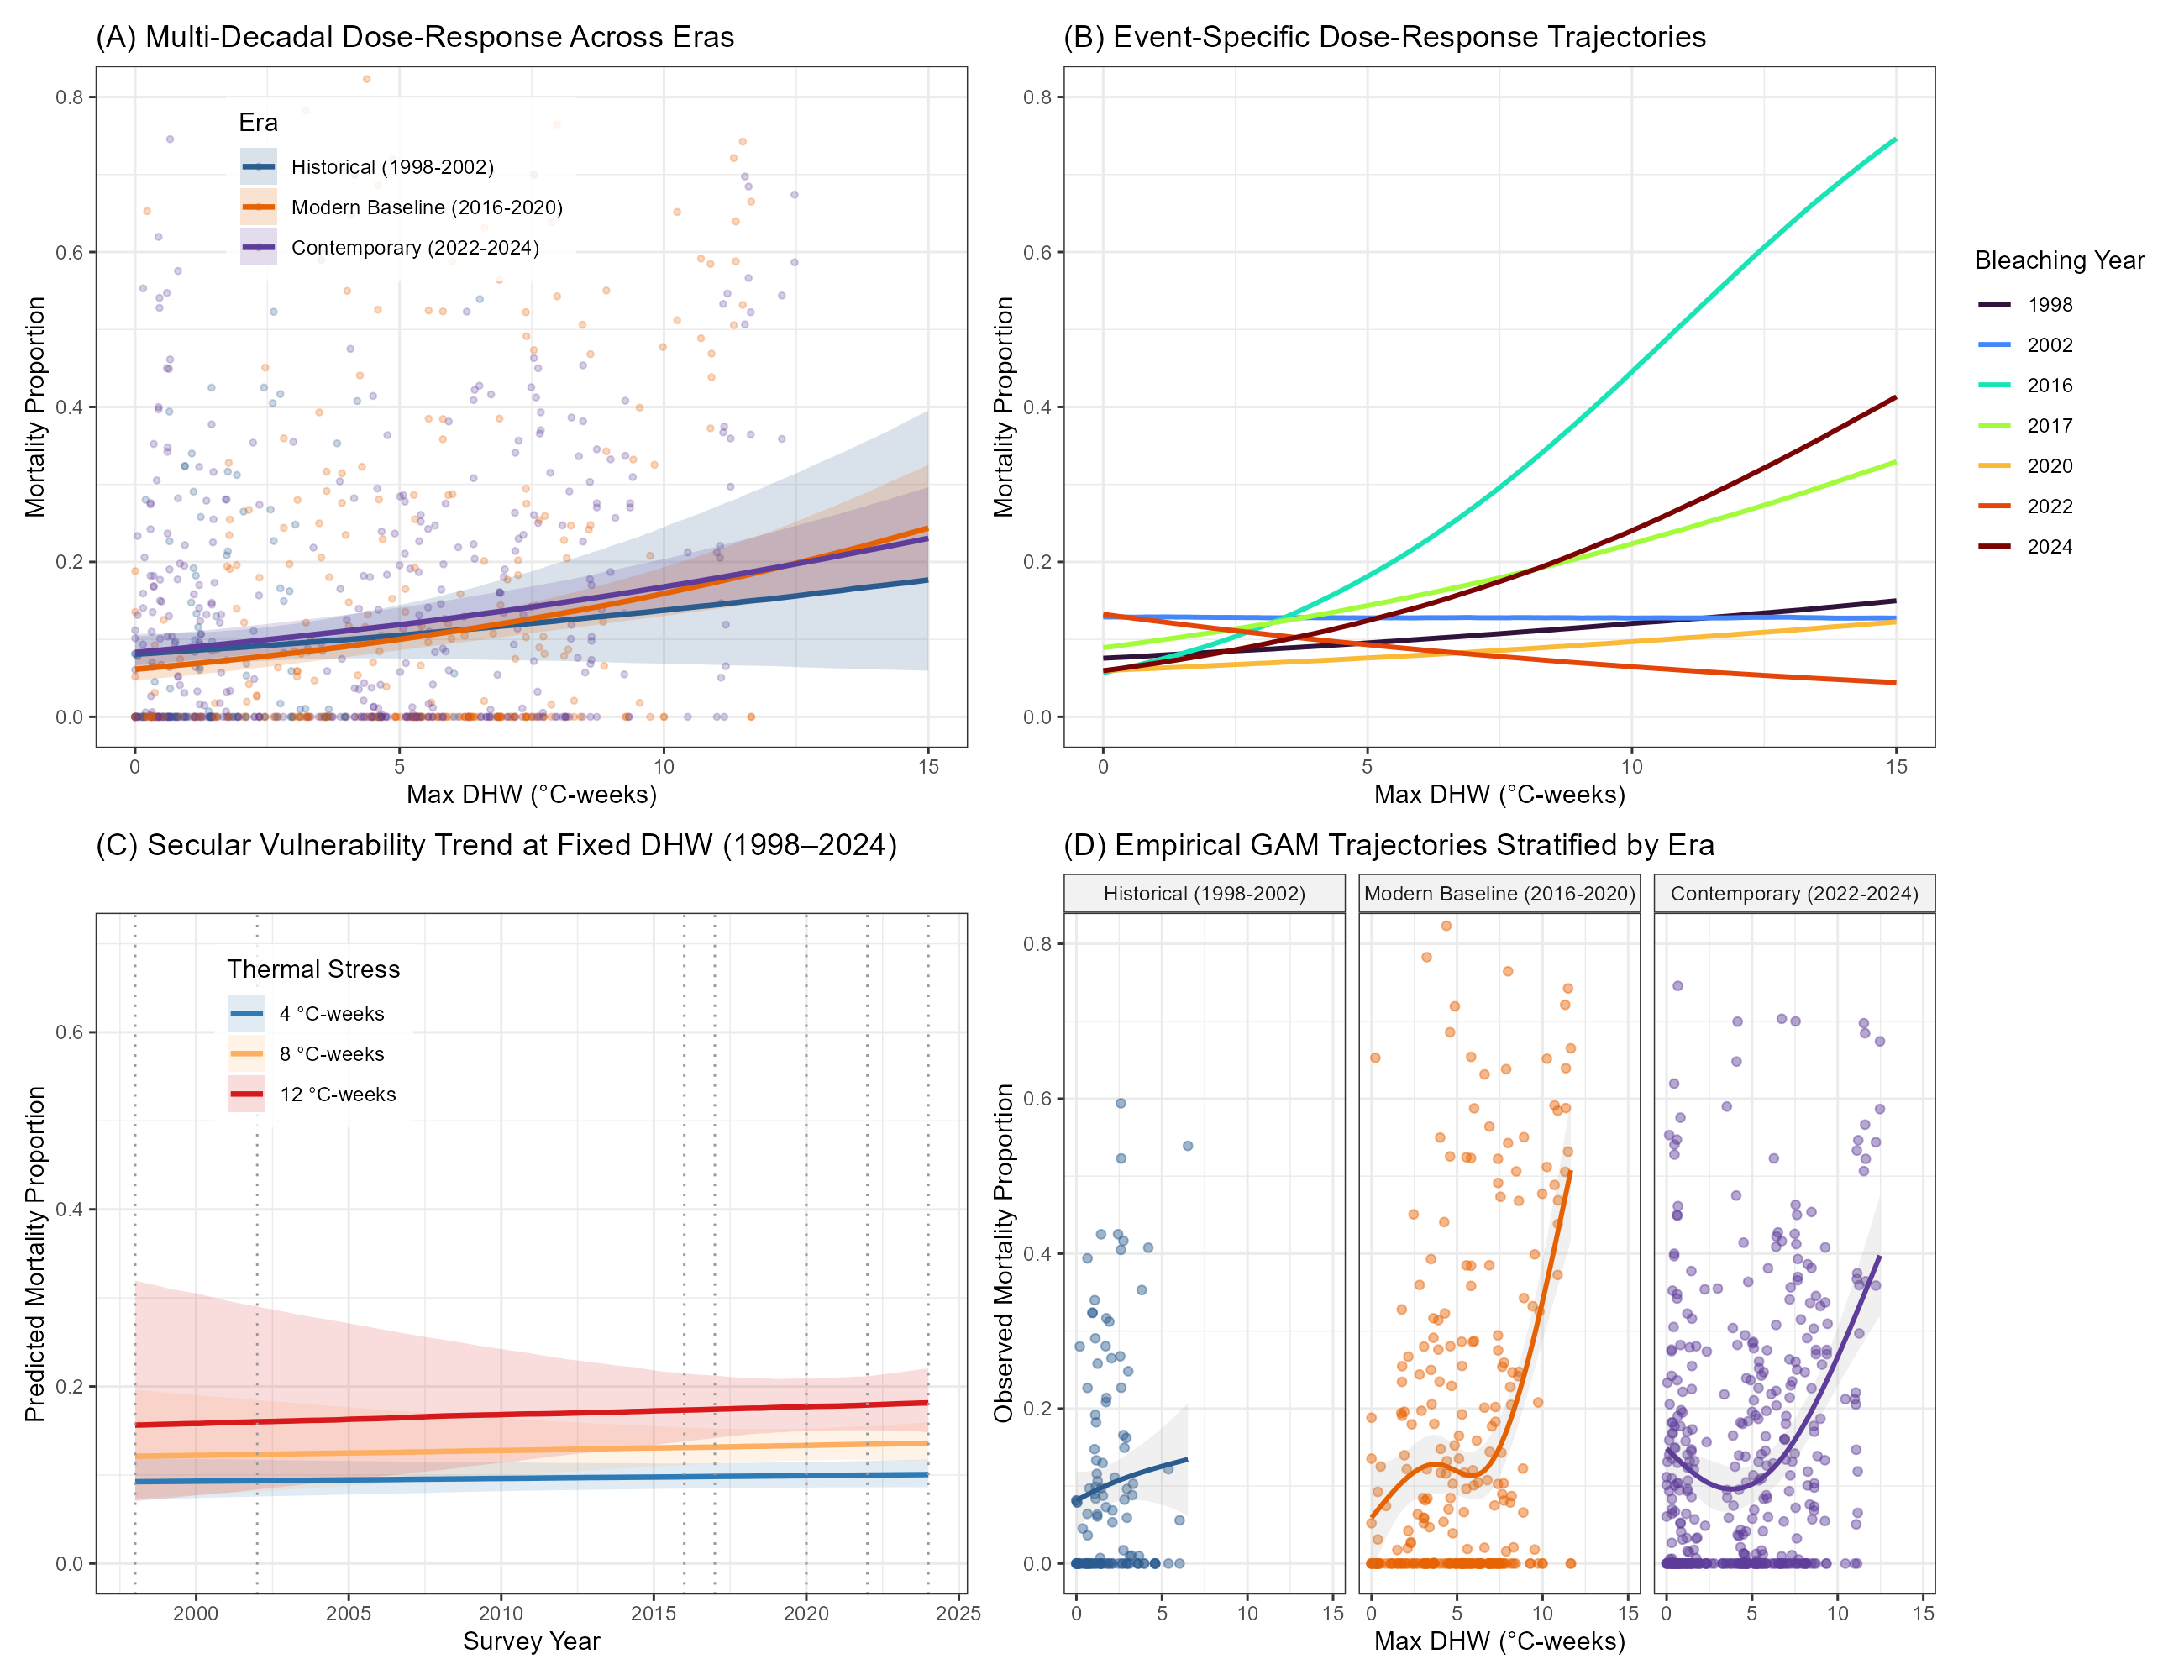
\includegraphics[width=8.67in,height=\textheight,keepaspectratio]{../output/plots/multidecadal_era_temporal_comparison.png}

}

\caption{\label{fig-dose-response}Bayesian dose-response mortality
trajectories across distinct historical bleaching eras and localized
environmental buffering contexts.}

\end{figure}%

\begin{figure}

\centering{

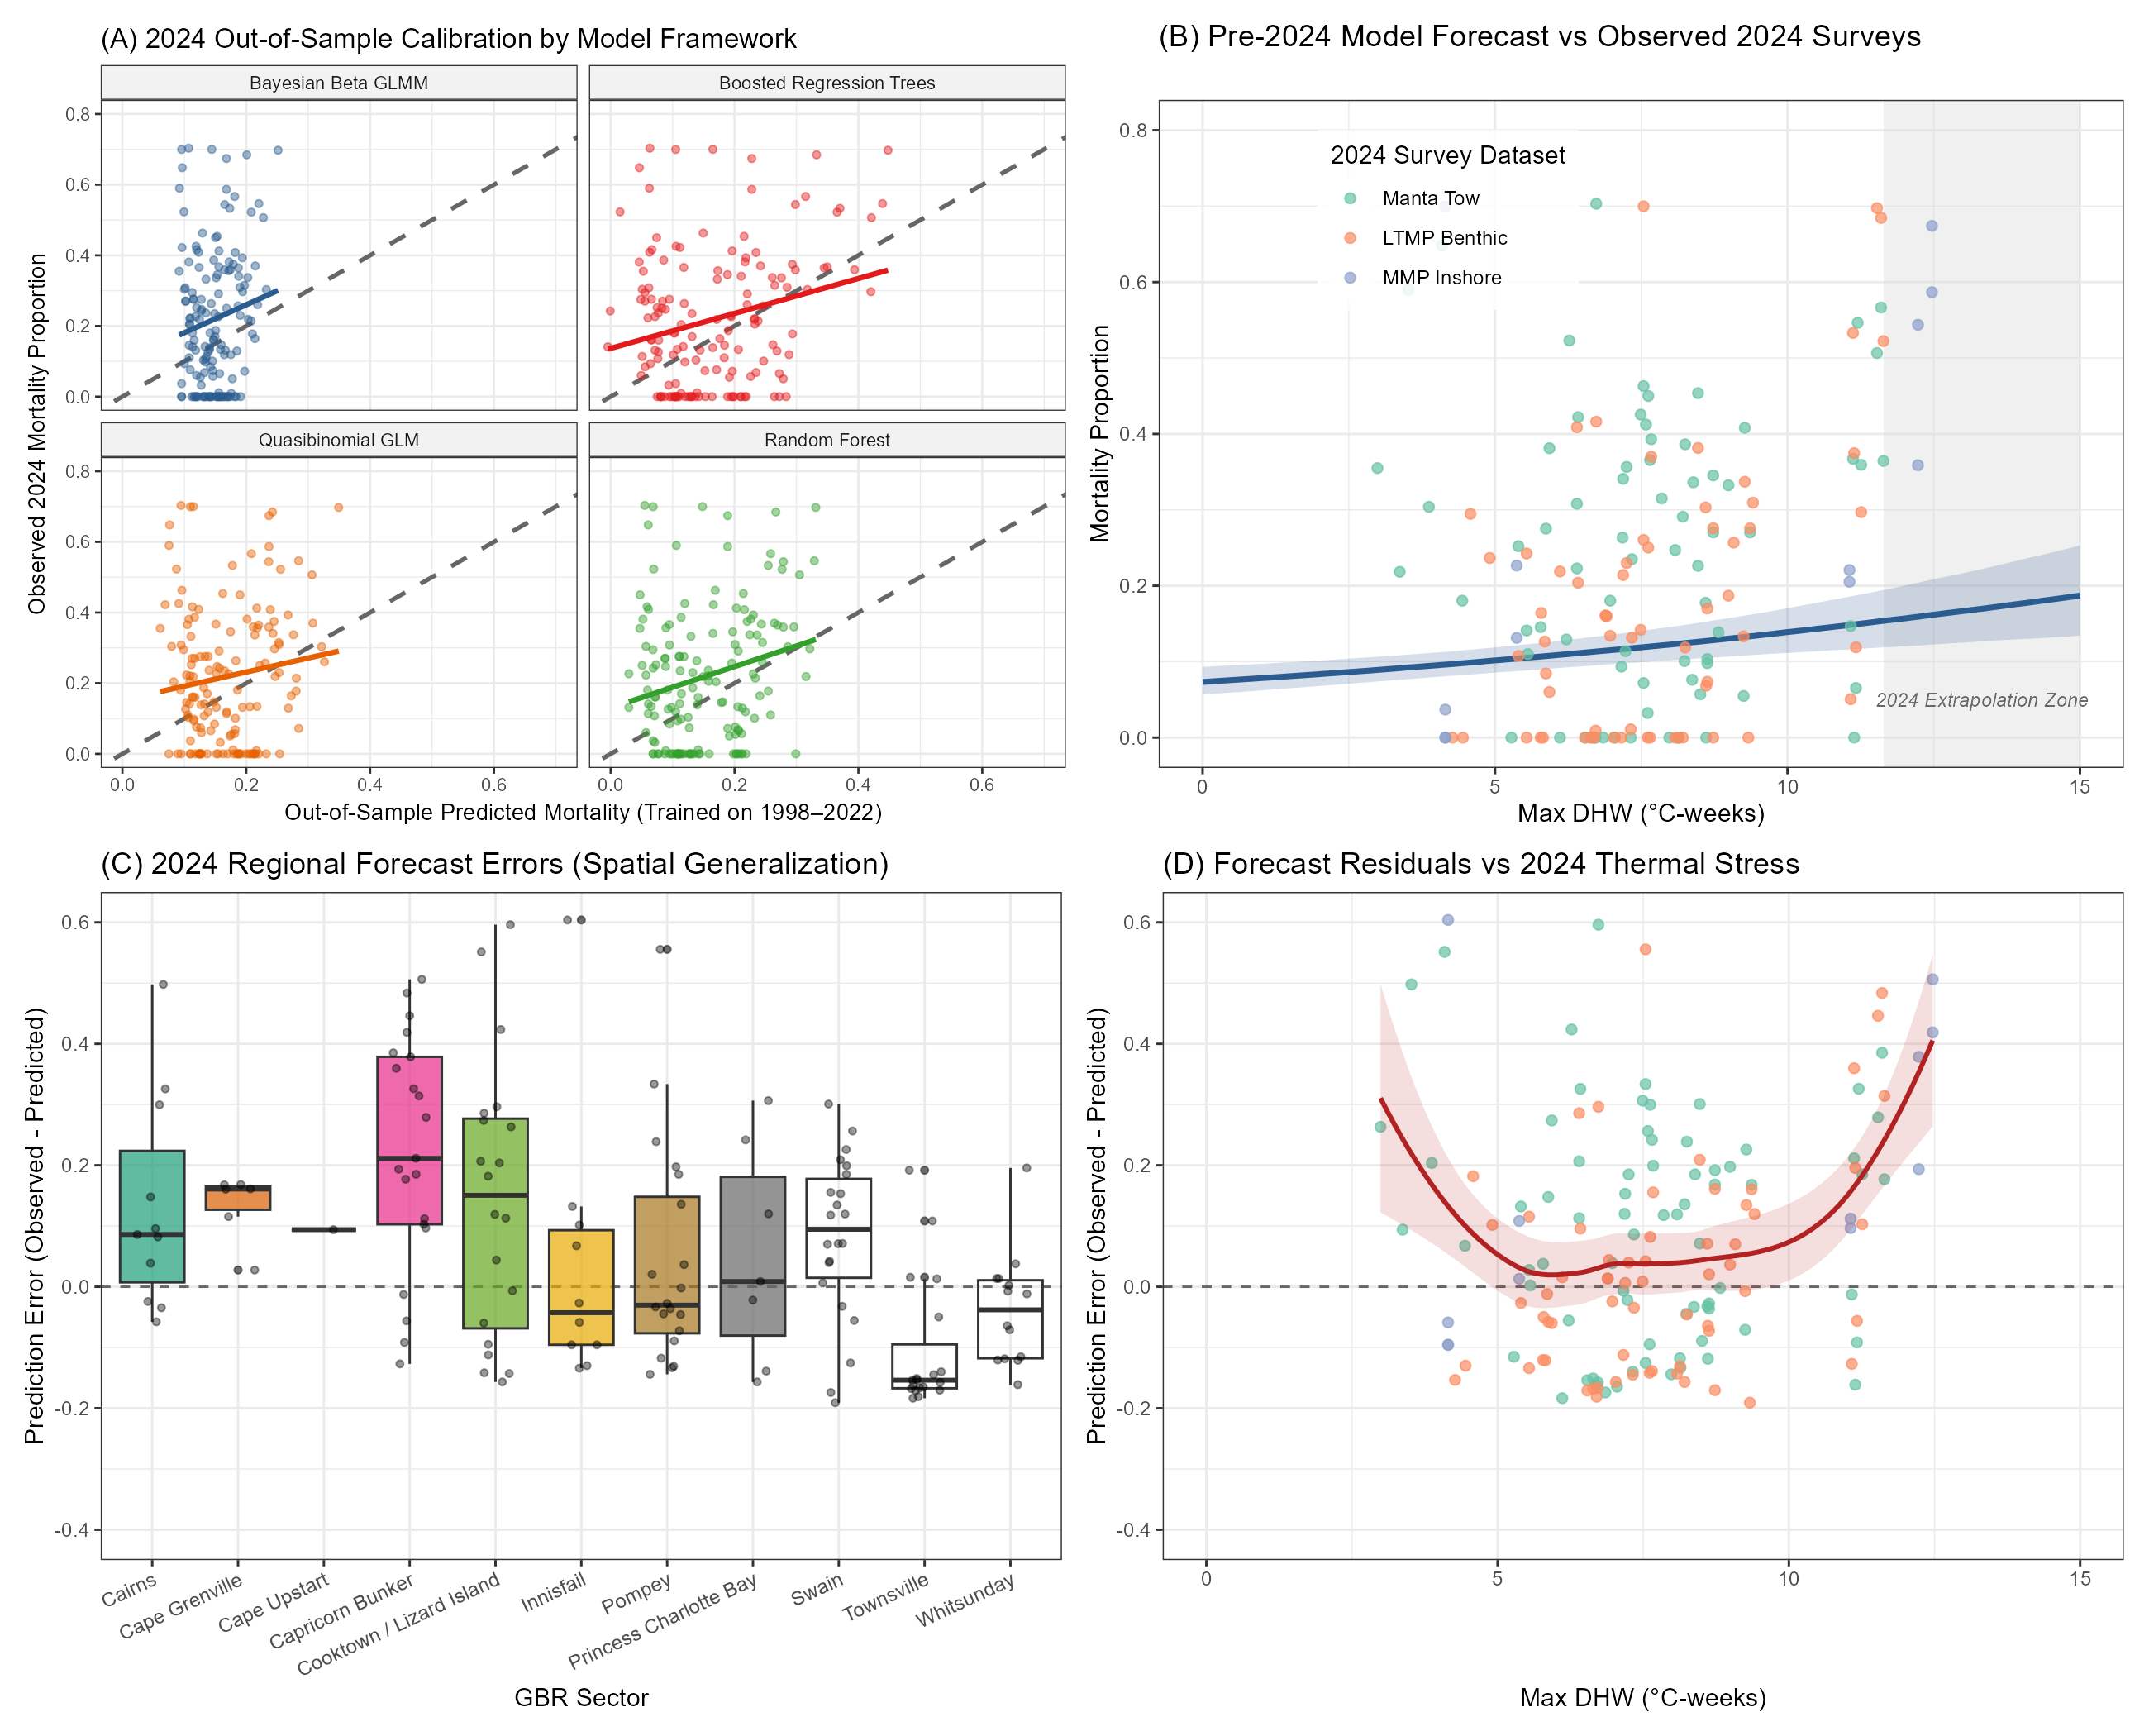
\includegraphics[width=8.67in,height=\textheight,keepaspectratio]{../output/plots/traintest_2024_out_of_sample_evaluation.png}

}

\caption{\label{fig-2024-out-of-sample}Out-of-sample predictive
performance stress-testing the model architecture against the extreme
2024 mass bleaching anomaly.}

\end{figure}%

\section{Discussion}\label{discussion}

Treating the Great Barrier Reef as a homogenous thermal surface obscures
the fine-scale physical and biological contexts that dictate coral
survival. Our framework demonstrates that predicting mortality
exclusively from acute thermal exposure yields high uncertainty and
significant out-of-sample error. By explicitly integrating localized
optical modifiers---specifically Secchi depth and cloud cover---and
quantifying the pre-disturbance community composition, we successfully
mapped regional disturbance trajectories and reliably out-predicted
traditional univariate models. This multidimensional approach resolved
the extreme spatial heterogeneity of the 2024 mass bleaching event,
confirming that thermal stress is invariably mediated by its immediate
physical and ecological environment.

The severe penalty associated with high pre-disturbance \emph{Acropora}
cover (\(\beta = 0.58\)) quantifies a known life-history trade-off at
the regional scale. Acroporids drive rapid architectural recovery
following disturbance but exhibit acute physiological sensitivity to
thermal anomalies (Marshall and Baird 2000). Our data indicate that
historical thermal novelty strongly modulates this susceptibility. Reefs
subjected to repeated, sub-lethal stress events often shift toward more
thermally tolerant assemblages (Hughes et al. 2017; Pratchett,
McWilliam, and Riegl 2020). Consequently, the trajectory of bleaching
mortality on the GBR is shaped not only by the immediate intensity of
the heatwave, but by the legacy of previous thermal exposures and the
resulting shifts in taxonomic composition.

Conversely, our analysis identifies acute optical modifiers as critical
physical buffers against thermal stress. High localized cloud cover and
reduced water clarity severely attenuated mortality at extreme DHW
thresholds, corroborating the hypothesis that shading acts as a primary
refugium mechanism (Cacciapaglia and Woesik 2016). Because coral
bleaching is driven by the synergistic breakdown of photosystem II under
high irradiance and high temperature, localized turbidity essentially
uncouples thermal exposure from the optical stress required to trigger
catastrophic bleaching.

These spatial gradients in vulnerability translate directly into
pragmatic triage criteria for resilience-based management (Oppen et al.
2017). Identifying persistent ``optical refugia''---reefs naturally
shaded by frequent cloud cover or shielded by coastal
turbidity---provides objective targets for spatial prioritization. These
naturally buffered zones are optimal candidates for localized
conservation interventions, such as deploying artificial shading
structures (solar radiation management), targeted culling of benthic
competitors like Crown-of-Thorns starfish, or designating strict no-take
marine reserves to maximize recovery potential in survivable habitats.

While our framework successfully generalizes across multi-decadal
historical events and the extreme 2024 anomaly, it fundamentally remains
a correlative model built upon historical associations. Deterministic
future forecasting using this architecture assumes static thermal
tolerance and does not dynamically simulate rapid evolutionary
adaptation, epigenetic acclimation, or shifting functional thresholds
under continuous, chronic warming (Hughes et al. 2018). Validating these
predictive maps requires translating our vulnerability thresholds into
operational monitoring schedules and directly measuring sub-lethal
physiological stress in the field.

Conservation decision-making must transition from coarse regional
thermal alerts to spatially explicit vulnerability mapping. Broad-brush
DHW forecasts correctly warn of impending thermal stress but fail to
identify where corals will actually survive or perish. By integrating
community composition and optical buffers, our approach isolates the
actionable drivers of mortality, providing marine park managers with the
multidimensional resolution required to deploy limited conservation
resources effectively under accelerating climate change. \# References

\phantomsection\label{refs}
\begin{CSLReferences}{1}{0}
\bibitem[\citeproctext]{ref-cacciapaglia2016}
Cacciapaglia, Chris, and Robert van Woesik. 2016. {``Climate-Change
Refugia: Shading Reef Corals by Turbidity.''} \emph{Global Change
Biology} 22 (3): 1145--54. \url{https://doi.org/10.1111/gcb.13166}.

\bibitem[\citeproctext]{ref-eakin2019}
Eakin, C Mark, Hugh PA Sweatman, and Russell E Brainard. 2019. {``The
2014--2017 Global-Scale Coral Bleaching Event: Insights and Impacts.''}
\emph{Coral Reefs} 38 (4): 539--45.
\url{https://doi.org/10.1007/s00338-019-01844-2}.

\bibitem[\citeproctext]{ref-hughes2017}
Hughes, Terry P, James T Kerry, Mariana Álvarez-Noriega, Jorge G
Álvarez-Romero, Kristen D Anderson, Andrew H Baird, Russel C Babcock, et
al. 2017. {``Global Warming and Recurrent Mass Bleaching of Corals.''}
\emph{Nature} 543 (7645): 373--77.

\bibitem[\citeproctext]{ref-hughes2018}
Hughes, Terry P, James T Kerry, Andrew H Baird, Sean R Connolly, Andreas
Dietzel, C Mark Eakin, Scott F Heron, et al. 2018. {``Spatial and
Temporal Patterns of Mass Bleaching of Corals in the Anthropocene.''}
\emph{Science} 359 (6371): 80--83.
\url{https://doi.org/10.1126/science.aan8048}.

\bibitem[\citeproctext]{ref-macneil2019}
MacNeil, M Aaron, Camille Mellin, Samuel Matthews, Nicholas H Wolff, Tim
R McClanahan, Michelle Devlin, Christopher Drovandi, Kerrie Mengersen,
and Russ C Babcock. 2019. {``Water Quality Mediates Resilience on the
Great Barrier Reef.''} \emph{Nature Ecology \& Evolution} 3 (4):
620--27. \url{https://doi.org/10.1038/s41559-019-0832-3}.

\bibitem[\citeproctext]{ref-marshall2000}
Marshall, Paul A, and Andrew H Baird. 2000. {``Bleaching of Corals on
the Great Barrier Reef: Differential Susceptibilities Among Taxa.''}
\emph{Oecologia} 122 (3): 355--61.

\bibitem[\citeproctext]{ref-vanoppen2017}
Oppen, Madeleine JH van, Ruth D Gates, Linda L Blackall, Neal Cantin,
Leela J Chakravarti, Wing Y Chan, Craig Cormick, et al. 2017.
{``Shifting Paradigms in Restoration of the World's Coral Reefs.''}
\emph{Global Change Biology} 23 (9): 3437--48.
\url{https://doi.org/10.1111/gcb.13647}.

\bibitem[\citeproctext]{ref-pratchett2020}
Pratchett, Morgan S, Michael J McWilliam, and Bernhard Riegl. 2020.
{``Changes in Bleaching Susceptibility Among Corals Subject to Ocean
Warming and Recurrent Bleaching in the Maldives.''} \emph{Nature
Communications} 11 (1): 712.

\bibitem[\citeproctext]{ref-safaie2018}
Safaie, Aryan, Nyssa J Silbiger, Tim R McClanahan, Geno Pawlak, Daniel J
Barshis, James L Hench, Justin S Rogers, Gareth J Williams, and Kristen
A Davis. 2018. {``High-Frequency Temperature Variability Reduces the
Risk of Coral Bleaching.''} \emph{Nature Communications} 9 (1): 1671.
\url{https://doi.org/10.1038/s41467-018-04074-2}.

\bibitem[\citeproctext]{ref-wold2023}
Wold, Renee, Jacquelyn Simpson, Spencer Miller, Joshua R Hancock,
Crawford Drury, and Joshua S Madin. 2023. {``Fine-Scale Variability in
Coral Bleaching and Mortality During a Marine Heatwave.''}
\emph{Frontiers in Marine Science} 10: 1108365.
\url{https://doi.org/10.3389/fmars.2023.1108365}.

\end{CSLReferences}




\end{document}
